\subsection{题目描述}
\noindent The table below gives the temperature \( T \) along a metal rod whose ends are kept at fixed constant temperatures. The temperature is a function of the distance \( x \) along the rod.
\begin{itemize}
    \item[(1)] Compute a least-squares, straight-line fit to these data using \( T(x) = a + bx \).
    \item[(2)] Compute a least-squares, parabolic-line fit to these data using \( T(x) = a + bx + cx^2 \).
\end{itemize}


\begin{table}[H]
    \centering
    \caption{Temperature data along the metal rod}
    \begin{tabular}{@{}ccccccccccc@{}}
        \toprule
        \(x_i\) (cm) & 1.0 & 2.0 & 3.0 & 4.0 & 5.0 & 6.0 & 7.0 & 8.0 & 9.0 \\ 
        \midrule
        \(T_i\) (°C) & 14.6 & 18.5 & 36.6 & 30.8 & 59.2 & 60.1 & 62.2 & 79.4 & 99.9 \\ 
        \bottomrule
    \end{tabular}
\end{table}

\subsection{程序描述}
本程序按照以下流程执行:先使用 \texttt{np.vstack} 函数垂直堆叠数组,构建设计矩阵。两个模型分别为
\[
A_{\text{linear}} = \begin{bmatrix} 1 & 1 & \cdots & 1 \\ x_1 & x_2 & \cdots & x_n \end{bmatrix}^T, A_{\text{quadratic}} = \begin{bmatrix} 1 & 1 & \cdots & 1 \\ x_1 & x_2 & \cdots & x_n \\ x_1^2 & x_2^2 & \cdots & x_n^2 \end{bmatrix}^T
\]
然后,对设计矩阵进行SVD(\textit{本程序的SVD分解借助\texttt{numpy}库实现}),即\(A = U \Sigma V^T\)
其中 \( U \) 和 \( V \) 是正交矩阵,\( \Sigma \) 是对角矩阵,包含奇异值 \( \sigma_1, \sigma_2, \dots, \sigma_p \),其中 \( p = \min(m, n) \)。为了计算Moore-Penrose伪逆 \( A^+ \),首先要对奇异值进行处理,将接近零的奇异值的倒数\textbf{简单截断},即
\[
\sigma_i^+ = 
\begin{cases}
\frac{1}{\sigma_i}, & \text{if } \sigma_i > \tau \\
0, & \text{otherwise}
\end{cases}
\]
本程序中阈值 \( \tau = 1 \times 10^{-10} \)。构建 \( \Sigma^+ \) 矩阵后,伪逆矩阵 \( A^+ \) 通过以下公式计算:\(A^+ = V \Sigma^+ U^T\)
利用伪逆矩阵,可以求解最小二乘问题的参数向量 \( \boldsymbol{\beta} \),即\(
\boldsymbol{\beta} = A^+ T\).
这种正则化步骤减少了因奇异值接近零而可能导致的数值不稳定,降低了对噪声的敏感性。\textbf{岭回归}也是一种常用的正则化方法,通过在最小二乘目标函数中加入 \( L^2 \) 正则化项,
\[
\min_{\boldsymbol{\beta}} \| A\boldsymbol{\beta} - T \|_2^2 + \lambda \| \boldsymbol{\beta} \|_2^2
\]
其中 \( \lambda \) 是正则化参数,其解析解为\(\boldsymbol{\beta}_{\text{ridge}} = (A^T A + \lambda I)^{-1} A^T T\),其有效地减小了参数的方差,提升了模型在新数据上的泛化能力。但本程序没有用此牛刀。在\texttt{src}目录使用\ccmd{python -u least\_squares.py}即可运行。
\subsection{伪代码}
\begin{algorithm}[H]
\caption{Pseudo-inverse computation and model fitting}
\KwIn{$x(\text{array}, \text{shape}=n)$, $T(\text{array}, \text{shape}=n)$}
\KwOut{$\beta(\text{array})$, $T_{\text{fit}}(\text{array})$, $RSS(float)$}

\SetKwFunction{pseudoInverse}{compute\_pseudo\_inverse}

$A_{\text{linear}} \leftarrow \begin{bmatrix} 1 & 1 & \cdots & 1 \\ x_1 & x_2 & \cdots & x_n \end{bmatrix}^T$, 
$A_{\text{quadratic}} \leftarrow \begin{bmatrix} 1 & 1 & \cdots & 1 \\ x_1 & x_2 & \cdots & x_n \\ x_1^2 & x_2^2 & \cdots & x_n^2 \end{bmatrix}^T$  \tcp*[r]{Design matrices for fits}

\SetKwProg{Fn}{Function}{:}{end}
\Fn{\pseudoInverse{$A$}}{
    $U, \Sigma , V^T \leftarrow \texttt{np.linalg.svd}(A, \text{full\_matrices=False})$ \tcp*[r]{Compute SVD of $A$}
    \ForEach{$\Sigma_i \in \Sigma$}{
        \eIf{$\Sigma_i > 10^{-10}$}{
            $\Sigma_{\text{inv}}[i] \leftarrow \frac{1}{\Sigma_i}$
        }{
            $\Sigma_{\text{inv}}[i] \leftarrow 0$
        }
    }
    $\Sigma_{\text{inv}} \leftarrow \text{diag}(\Sigma_{\text{inv}})$
    $A^+ \leftarrow V^T \cdot \Sigma_{\text{inv}} \cdot U^T$
    \KwRet{$A^+$}
}
$\beta \leftarrow A^+ T$;$T_{\text{fit}} \leftarrow \sum_{i=0}^{d} \beta_i x^i$ ;$RSS \leftarrow \sum(T - T_{\text{fit}})^2$ \tcp*[r]{Compute residual sum of squares (RSS)}


\KwRet{$\beta_{\text{linear}}, T_{\text{fit, linear}}, RSS_{\text{linear}}$, $\beta_{\text{quadratic}}, T_{\text{fit, quadratic}}, RSS_{\text{quadratic}}$}
\end{algorithm}
    
    


\subsection{结果示例}
\begin{figure}[H]
    \centering
    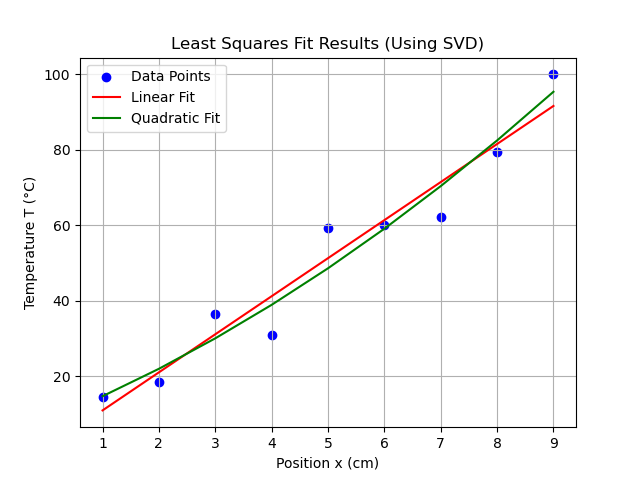
\includegraphics[width=1.0\textwidth]{Problem_2/figs/plot.png}
    \caption{拟合结果}
\end{figure}

\begin{figure}[H]
    \centering
    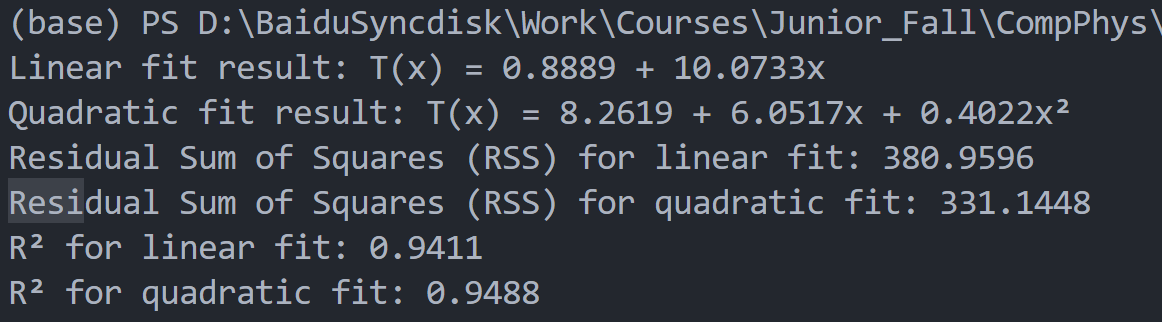
\includegraphics[width=1.0\textwidth]{Problem_2/figs/result.png}
    \caption{终端输出}
\end{figure}
